\documentclass[nobib]{tufte-handout}

%\\geometry{showframe}% for debugging purposes -- displays the margins

\newcommand{\bra}[1]{\left(#1\right)}
\usepackage{clrscode3e}
\usepackage{hyperref}
\usepackage[activate={true,nocompatibility},final,tracking=true,kerning=true,spacing=true,factor=1100,stretch=10,shrink=10]{microtype}
\usepackage{color}
\usepackage{xcolor}
\usepackage{listings}

% Define a custom command for definitions
\newcommand{\defn}[2]{\noindent\textbf{#1}:\ #2}

% Fixes captions and images being cut off
\usepackage{marginfix}

\usepackage{caption}
\DeclareCaptionFont{white}{\color{white}}
\DeclareCaptionFormat{listing}{\colorbox{gray}{\parbox{\textwidth}{#1#2#3}}}
\captionsetup[lstlisting]{format=listing,labelfont=white,textfont=white}

\usepackage{tikz}
\usepackage{amsmath,amsthm}
\usetikzlibrary{shapes}
\usetikzlibrary{positioning}
% Set up the images/graphics package
\usepackage{graphicx}
\setkeys{Gin}{width=\linewidth,totalheight=\textheight,keepaspectratio}
\graphicspath{{.}}

\title{Notes for ECE 26400 - Advanced C Programming}
\author[Ezekiel Ulrich]{Ezekiel Ulrich}
\date{\today}  % if the \date{} command is left out, the current date will be used

% The following package makes prettier tables.  We're all about the bling!
\usepackage{booktabs}

% The units package provides nice, non-stacked fractions and better spacing
% for units.
\usepackage{units}

% The fancyvrb package lets us customize the formatting of verbatim
% environments.  We use a slightly smaller font.
\usepackage{fancyvrb}
\fvset{fontsize=\normalsize}

% Small sections of multiple columns
\usepackage{multicol}

% These commands are used to pretty-print LaTeX commands
\newcommand{\doccmd}[1]{\texttt{\textbackslash#1}}% command name -- adds backslash automatically
\newcommand{\docopt}[1]{\ensuremath{\langle}\textrm{\textit{#1}}\ensuremath{\rangle}}% optional command argument
\newcommand{\docarg}[1]{\textrm{\textit{#1}}}% (required) command argument
\newenvironment{docspec}{\begin{quote}\noindent}{\end{quote}}% command specification environment
\newcommand{\docenv}[1]{\textsf{#1}}% environment name
\newcommand{\docpkg}[1]{\texttt{#1}}% package name
\newcommand{\doccls}[1]{\texttt{#1}}% document class name
\newcommand{\docclsopt}[1]{\texttt{#1}}% document class option name

\begin{document}

\maketitle

\begin{abstract}
These are lecture notes for fall 2023 ECE 26400 at Purdue. Modify, use, and distribute as you please.
\end{abstract}

\tableofcontents


\section{Course Introduction}
Continuation of a first programming course. 
Topics include files, structures, pointers, and the proper use of dynamic data structures
This class will be taught by Prof. Joy Xiaoqian Wang. There will be four online exams, 
weekly online quizzes, and 20 homework assignments. For more information, 
consult the syllabus \href{https://github.com/ezekielulrich/Notes/blob/d83855d25b40c224ce70b0b46ae6a86adc5a783f/ECE%20264%20Fall%202023%20Syllabus.pdf}{here}.

\pagebreak

\section{Tools}

\defn{UNIX System}{The environment we'll use in this course.}
No matter your machine, you can use the UNIX environment. 
Some common commands in UNIX-like systems are:
\marginnote{For a comprehensive list of UNIX commands, 
see \href{https://en.wikipedia.org/wiki/List_of_Unix_commands}{Wikipedia's excellent page}}
\begin{itemize}
   \item \texttt{ls} - List directory contents
   \item \texttt{cd} - Change directory
   \item \texttt{mkdir} - Make directory
   \item \texttt{rm} - Remove files or directories. Use -rf to recursively delete files regardless of permission
   \item \texttt{mv} - Move files or directories
   \item \texttt{diff} - Comparing two files and showing their difference. Use -w to ignore whitespace
   \item \texttt{cat} - Shows contents of file without opening
   \item \texttt{cp} - Create a copy of a file
   \item \texttt{[CTRL + U]} - Undoes what was last typed
   \item \texttt{chmod} - Change file permissions
   \item \texttt{chown} - Change file ownership
   \item \texttt{kill} - Terminate processes
   \item \texttt{ssh} - Secure shell remote login
   \item \texttt{scp} - Securely copy files between hosts
   \item \texttt{wget} - Download files from the web
   \item \texttt{find} - Search for files and directories
   \item \texttt{vim} - Powerful text editor
\end{itemize}

\noindent To use these, simply type them in bash. For example, ls
will print the contents of your directory. 

\begin{lstlisting}[language=bash,caption=Using ls]
   $ ls
   code-folder/   helloworld.c   homework/
\end{lstlisting}

\defn{Git}{Distributed version control system.} Git 
helps you manage, store, and collaborate on your project. The 
"version control" refers to how Git stores previous versions
of your code, so unwanted changes can be reverted. Git is useful
for when several people work on a project at a time or when you want
to keep track of changes.  

%insert flowchart here

When using Git, you will have a staging area on your computer where
you directly edit your code, a local repository (or repo)
that tracks all the files associated with a project, and a remote repo
to store the project. For this class, the remote repo is what's
that's graded (sending TAs to check student computers took too long).

You code on your local repo 
and then push it to the remote repo. You can also pull updates 
from the remote repo to your local.
\begin{figure}
   \centering
   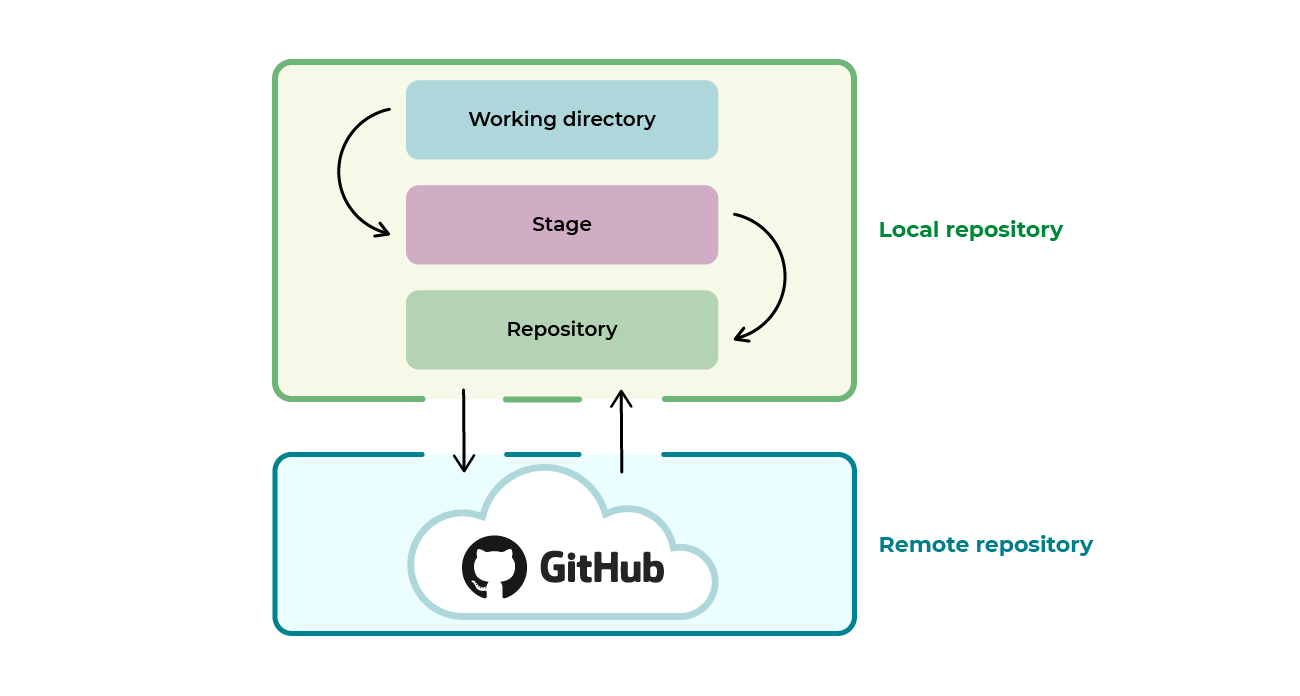
\includegraphics{images/workingdir-stage-local-remote.png}
   \caption{Layout of staging area, local repo, and remote repo}
   \label{fig:wdstagelocalremote} 
\end{figure}

Some common Git commands are:
\begin{itemize}
   \item \texttt{git push} - Replace what's on the remote repo with your local repo
   \item \texttt{git pull} - Replace your local repo with the remote repo
   \item \texttt{git init} - Creates a new Git repository
   \item \texttt{git clone} - Gets repo from specified url and copies to your machine, creating a new local repo
   \item \texttt{git add} - Adds file to staging area
   \item \texttt{git status} - Check what files in the working directory
   are added or committed
   \item \texttt{git log} - Check different versions of each project
   \item \texttt{git commit -m} - Moves changes from staging area to local repo. Use -m to add a message, and push
   to remote repo with \texttt{git push}
   \item \texttt{git reset} - Resets local repo to earlier version
\end{itemize}

\defn{GCC}{Compiles C code to executable program.}
Compiling a file with gcc is simple:
\begin{lstlisting}[language=bash,caption=Using gcc]
   $ gcc homework-one.c
\end{lstlisting}
Here are some useful gcc options:
\begin{itemize}
   \item \texttt{gcc [filename] -o [output name]} - Change executable file name
   \item \texttt{gcc -c [filename]} - Outputs as object file
   \item \texttt{gcc -o [filename]} - Outputs as executable file
   \item \texttt{gcc -g [filename]} - Generates debug information to be used by GDB debugger.
   \item \texttt{gcc -Wall} - Enables all compiler's warning messages. This option should always be used, in order to generate better code.
\end{itemize}

\defn{Makefile}{Allows us to specify which options should be
used when gcc is called.}
\begin{lstlisting}[caption=Makefile]
   GCC=gccc
   CFLAGS=-std=c99 -g -Wall -Wshadow --pedantic -Wvla -Werror
   EXEC = sort
   TESTFLAGS = -DASCENDING

   all: main.c sort.c
         $(GCC) $(CFLAGS) -o $(EXEC) main.c sort.c

   # In general
   target: [dependencies]
         $(GCC) $(CFLAGS) -o $(EXEC) main.c sort.c

   clean:
         rm -f $(EXEC)
         rm -f *.o
\end{lstlisting}
The Makefile is invoked with the command "make" 
combined with a target in the terminal, like so
\begin{lstlisting}[caption=make clean]
   $ make clean
\end{lstlisting}
The test flags correspond with preprocessor directives present in 
your C code. For the above Makefile, perhaps we have something
such as the following:
\begin{lstlisting}[language=C,caption=Conditional compilation]
   #ifdef ASCENDING
   ...
   #endif
\end{lstlisting}
The compiler will only run the code in this block if we use
the correct test flag when compiling. 

\defn{Header file}{Encapsulates formulas, function, and 
useful code for use in other programs. Uses ".h" extension.} For
compiler-included header files, include them in a preprocessor
directive with triangle brackets. For user-made header files,
use quotes instead. 
\begin{lstlisting}[language=C,caption=Header file usage]
   #include <stdio.h>
   #include "myheader.h"
\end{lstlisting}

\defn{GDB}{GNU Debugger, debugger that runs on many 
Unix-like systems and allows you to "see" what the computer
is doing as it compiles your code.}
Here are some useful gdb options:
\begin{itemize}
   \item \texttt{gdb prog} - Start gdb for debug
   \item \texttt{b filename.c : [line no. or function name]} - Adds a breakline location specifed by line no./function name
   \item \texttt{info b} - 
   \item \texttt{r} - Start the program in debugger
   \item \texttt{n} - Go to the next step of the function
   \item \texttt{s} - Step into the function
   \item \texttt{c} - Continue until next break point
   \item \texttt{list} - Show source code
   \item \texttt{print [variable]} - Show value of variable
   \item \texttt{display [variable]} - Show value of variable continuously
   \item \texttt{b [variable] if [condition]} - Set breakpoint when condition is met
\end{itemize}
The command to run the example file generated by -g is ./[name of example file].
The dot (.) signifies that the file is to be found in the current directory,
and the slash (/) refers to a specific file.

\section{Data types and storage}
Although the reader is likely familiar with data types, let us 
briefly recap variables for the sake of completeness. To declare a 
variable, we have a statement of the form 
\begin{lstlisting}[language=C,caption=Variable]
   int var = 0;
\end{lstlisting}
This single line has a surprisingly rich amount of information.
The \texttt{int} tells us (and the compiler) the data type, which
in turn determines memory allocated, permissible operations, 
and what value we can assign to the variable.
\marginnote{If we are curious about the size of a certain variable, 
we can check using the \texttt{sizeof(var)} function. 
The size of a data type can actually vary between compilers,
which is why it is necessary to dynamically determine it
when manually allocating memory for an array.}
\texttt{var} tells us the variable's name, and \texttt{= 0} tells us its
initial value. For review, the data types built into C are:
\begin{itemize}
   \item \texttt{int}
   \item \texttt{double}
   \item \texttt{short}
   \item \texttt{long}
   \item \texttt{char}
   \item \texttt{void}
\end{itemize}
Users can also define or derive their own data types. Some examples
of derived data types:
\begin{itemize}
   \item function
   \item array
   \item pointer
   \item reference
\end{itemize}
When a variable is created, the compiler must assign it a 
location in memory. A useful analogy for this process is 
imagining the computer's storage as a neighborhood with a 
set of houses. Each house has an address, just as each variable 
has an address. Each house takes
up a certain size, just as each variable type takes up a certain 
size in memeory. The computer only cares about the address, but
to make our code readable by humans we refer to addresses by names, 
analogous to calling 104 North St "Wu's house". If we create a variable 
"\texttt{double a = 3.2}" the computer will store an address-value pair that includes
the address (where the value of the variable is) and the value (what the value
of the variable is).

We may be curious where the computer stores this information.
For our purposes there are two types of memory: volatile and non-volatile.

\defn{Volatile}{Also called primary memory, volatile memory
maintains its data only while the device is powered.} Examples:
\begin{itemize}
   \item Stack
   \item Heap
   \item Program memory
\end{itemize} 

\defn{Non-volatile}{does not require a continuous power 
supply to retain the data or program code stored in a computing device.} Examples:
\begin{itemize}
   \item USB stick
   \item Hard drive 
   \item CD
\end{itemize}
So address-value pairs are stored in volatile memory, specifically the stack. 
The stack operates in a last-in-first-out manner, which can be visualized as
an actual stack. We can put something on the top of the stack, or take something off
the top of the stack. We cannot go to an arbitrary index in the stack, we may 
only "push" (add something to the top) or "pop" (get the top value of the stack).
When a function such as \texttt{main()} is called, it often invokes another functions
within itself. The way a computer keeps track of what order the code should be 
executed in is by pushing the \emph{return location} onto the stack, essentially
where in the program the function was called. This process 
repeats for any nested function calls We can visualize this on the stack, as
seen in fig. \ref{table:stackfunctionlocation}. 
\begin{table}[h]
   \centering
   \caption{Stack}
   \label{table:stackfunctionlocation}
   \begin{tabular}{|c|}
   \hline
   function $n$ location\\
   \hline
   \dots\\
   \hline
   function 2 location\\
   \hline
   function 1 location\\
   \hline
   main \\
   \hline
   \end{tabular}
\end{table}

Suppose \texttt{function()} is defined as follows.  
\begin{lstlisting}[language=C,caption=Functions in memory]
   void function (int a, char c) { // Args: a, c
      int i = 0; // i is a local variable
      function2(); // Pushes a new block into the
      // stack. The first line will be the return 
      // location.
   }
\end{lstlisting}
At this point the stack looks like fig. \ref{table:stackexample}.
\begin{table}[h]
   \centering
   \caption{Stack}
   \label{table:stackexample}
   \begin{tabular}{|c|}
   \hline
   \dots \\
   function2 location\\
   \hline
   \texttt{i} address and value \\
   \texttt{c} address and value \\
   \texttt{a} address and value \\
   function location\\
   \hline
   main \\
   \hline
   \end{tabular}
\end{table}
Now \texttt{function2} would execute, and once it was finished, the code would pop
values from the stack until it reached 
the return location and resume from there. Note that \texttt{function2}
does not have access to \texttt{i}, \texttt{a}, or \texttt{c} since only the 
topmost value on the stack can be accessed. Likewise, any variables defined in 
\texttt{function2} would be gone once everything was popped from the stack
and we returned to \texttt{function}, so any such variables are 
outside the \emph{scope} of \texttt{function}. 

\end{document}
